\chapter{Controlling drones}

\section{PID controller}
My first sub-task of BTP was to train a drone in simulation to go from point A to point B without much deviations, jerks and oscillations.
It can be achieve in two ways, one by pid controller and other by training a drone by reinforcement learning. 
Its important to understand PID controller approach first, later will discuss the RL based approach.
\subsection{Introduction}
\subsubsection{PID}
PID stands for Proportional, Integral, Derivative, it’s part of a flight controller software that reads the data from sensors and calculates how fast the motors should spin in order to retain the desired rotation speed of the aircraft.\cite{pidwiki}
\\
The goal of the PID controller is to correct the “error“, the difference between a measured value (gyro sensor measurement), and a desired set-point (the desired rotation speed). The “error” can be minimized by adjusting the control inputs in every loop, which is the speed of the motors.\cite{pid}
\\
There are 3 values in a PID controller, they are the P term, I term, and D term:
\\
"P" looks at present error –  the further it is from the set-point, the harder it pushes
\\"D" is a prediction of future errors – it looks at how fast you are approaching a set-point and counteracts P when it is getting close to minimize overshoot
\\"I" is the accumulation of past errors, it looks at forces that happen over time; for example if a quad constantly drifts away from a set-point due to wind, it will spool up motors to counteract it
\\
\begin{figure}[H]
    \centering
    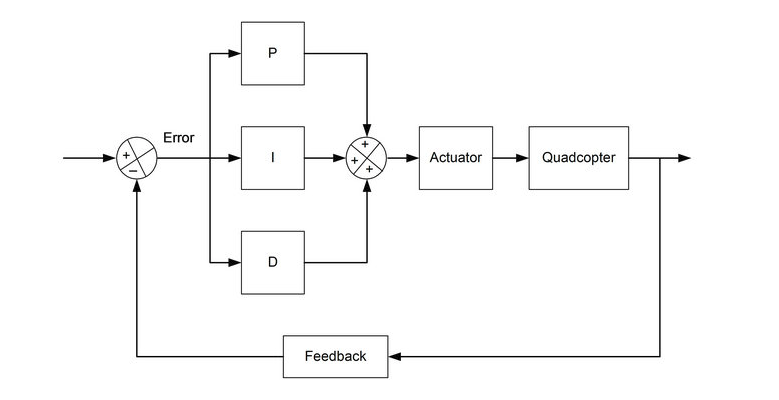
\includegraphics[width=\textwidth]{images/pid.png}
    \caption{PID Controller Diagram}
\end{figure}

\subsubsection{ROS}
Robot Operating System(ROS) is a meta-operating system for a robot. It provides services that one would expect from an operating system, including hardware abstraction, device drivers, libraries, visualizers, low-level device control, implementation of commonly-used functionality, message-passing between processes, and package management. It also provides tools and libraries for obtaining, building, writing, and running code across multiple computers. It is named as a meta-operating system because it is something between an operating system and middleware. It provides not only standard operating system services (like hardware abstraction) but also high-level functionalities like asynchronous and synchronous calls, a centralized database, a robot configuration system, etc. ROS can be interpreted also as a software framework for robot software development, providing the operating system. ROS is based on a Unix-like philosophy of building many small tools that are designed to work together. ROS grows out of a collaboration between industry and academia and is a novel blend of professional software development practices and the latest research results.\cite{ros}

\subsubsection{Pluto drone}
Drone used for this experiment is pluto drone, this is light weight drone. It have the support for ROS.\cite{plutoros}
\begin{figure}[H]
    \centering
    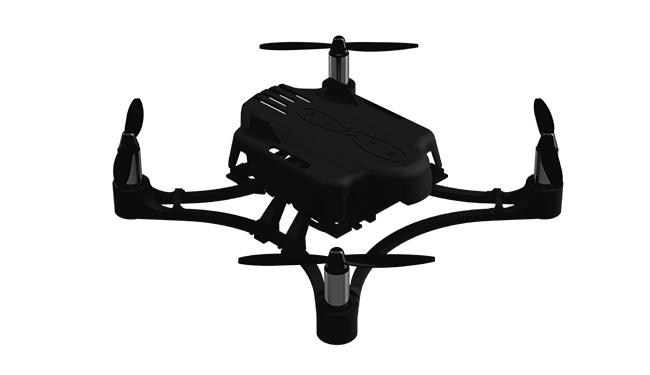
\includegraphics[width=0.5\textwidth]{images/pluto.png}
    \caption{Pluto drone}
\end{figure}

\subsubsection{V-REP}
V-REP is simulation software which can be used with ROS to simulated various robots.\cite{vrep}
\\
\newline \begin{figure}[H]
    \centering
    % \caption{V-Rep simulation of pluto drone}
    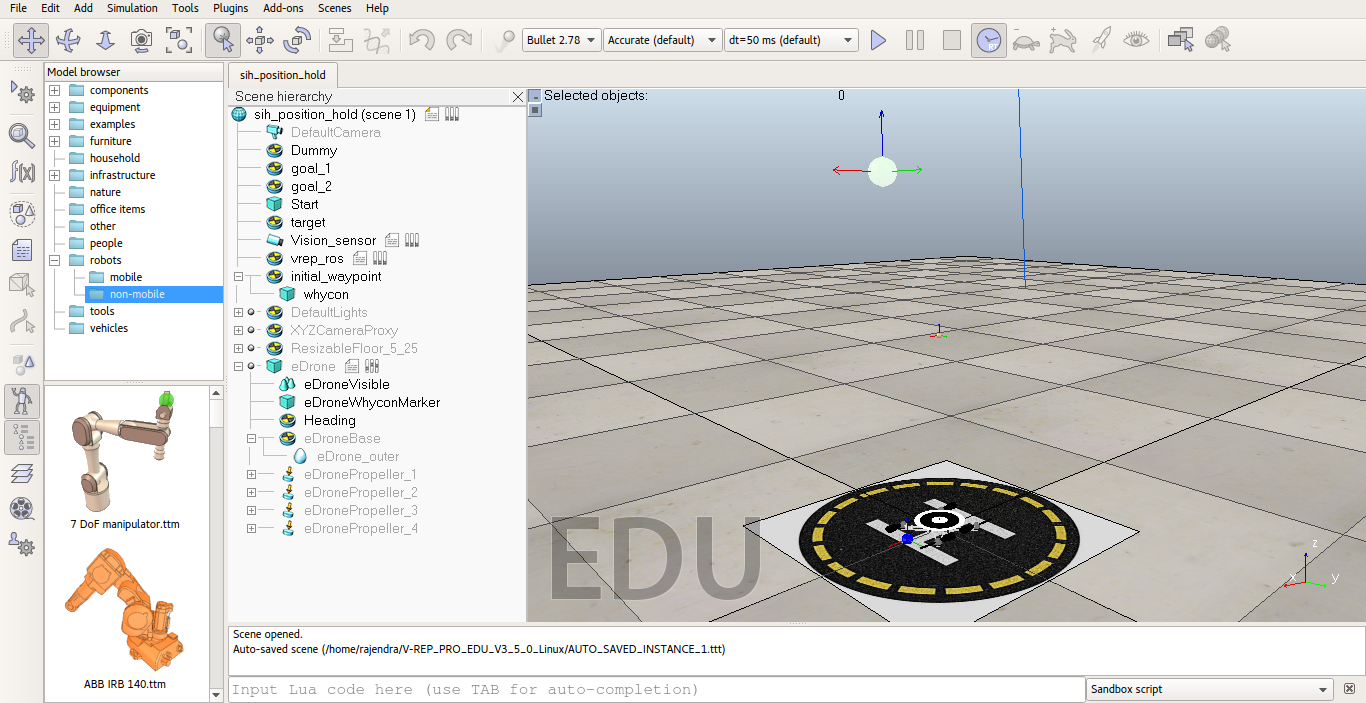
\includegraphics[width=\textwidth]{images/vrep.png}
    \\
    \caption{V-Rep simulation of pluto drone}
\end{figure}
\\
\subsection{Implementation}
Here we will implement the position hold algorithm for drone using ROS in vrep software.
\subsubsection{Algorithm}
\\
Lets describe the algorithm and pseudo code in brief. Full detailed code of the same can be found \href{https://github.com/iamrajee/Slam_and_RL_BTP/tree/master/code/pid}{here}. Here we uses the position of drone we get by detecting the whycon marker on the drone and publish the drone command to hold to the given position.
% \documentclass{article}

 
% \begin{document}
\begin{minted}{python}

	'''-------------------- PID algorithm here --------------'''
	# Steps:
	# 	1. Compute error in each axis. eg: error[0] = self.drone_position[0] - self.setpoint[0] ,where error[0] corresponds to error in x...
	#	2. Compute the error (for proportional), change in error (for derivative) and sum of errors (for integral) in each axis.
	#	3. Calculate the pid output required for each axis. For eg: calcuate self.out_roll, self.out_pitch, etc.
	#	4. Reduce or add this computed output value on the avg value ie 1500.EXPERIMENT AND FIND THE CORRECT SIGN
	#	5. Don't run the pid continously. Run the pid only at the a sample time. self.sampletime defined above is for this purpose.
	#	6. Limit the output value and the final command value between the maximum(1800) and minimum(1200)range before publishing.
	#	7. Update previous errors.eg: self.prev_error[1] = error[1] where index 1 corresponds to that of pitch
	#	8. Add error_sum
	
	'''--------------- PID algorithm code here---------------'''
	def pid(self):
		error = [0.0, 0.0, 0.0, 0.0] #reset every time
		change_in_error = [0.0, 0.0, 0.0, 0.0] #reset every time
		for i in range (0, 4):
			error[i] = self.setpoint[i] - self.drone_position[i] #find error
			self.error_pub[i].publish(error[i]) #publish error
			change_in_error[i] = error[i] - self.prev_values[i] #change in error
			self.sum_of_error[i] = self.sum_of_error[i] + error[i] #sum of error
			self.iterm[i] = self.iterm[i] + (error[i] * self.Ki[i]) #integral term
			self.output[i] = (self.Kp[i] * error[i]) + self.iterm[i] + (self.Kd[i] * change_in_error[i]) #all together
			self.prev_values[i] = error[i] 
		
		# set drone command based on current output error
		self.cmd.rcPitch = 1500 - self.output[0]
		self.cmd.rcRoll = 1500 - self.output[1]
		self.cmd.rcThrottle = 1500 - self.output[2]
		self.cmd.rcYaw = 1500 + self.output[3]
		
		self.setRange() #check if in range
		
		self.command_pub.publish(self.cmd) #publish command to drone

\end{minted}

\subsection{Conclusion}

I was able to hold the drone to given position but it required a lot and very precise pid tuning to get there.
Hence, PID control based algorithm is easy and intuitive to understand but hard to improve and tune.



















\section{Reinforcement Learning}
\subsection{Introduction}
Here we will try to implement the q learning based controller for drone in ros. Lets try to send drone from point A to B.
\subsubsection{ARdrone}
ARdrone most popular drone often used with the simulation using the ros.\cite{ardrone}
\begin{figure}[H]
    \centering
    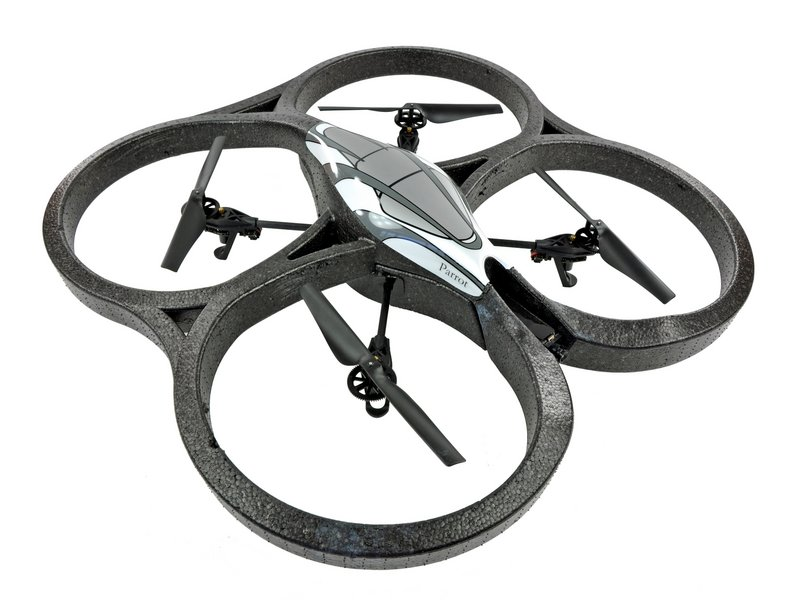
\includegraphics[width=0.5\textwidth]{images/ardrone.jpg}
    \caption{Ardrone}
\end{figure}
\subsubsection{ROS development studio}
I used the online ros development studio by \textbf{theconstruct} for simulating RL algorithm on the drone as my local system was not powerful enough to take heavy load.\cite{rds}

\begin{figure}[H]
    \centering
    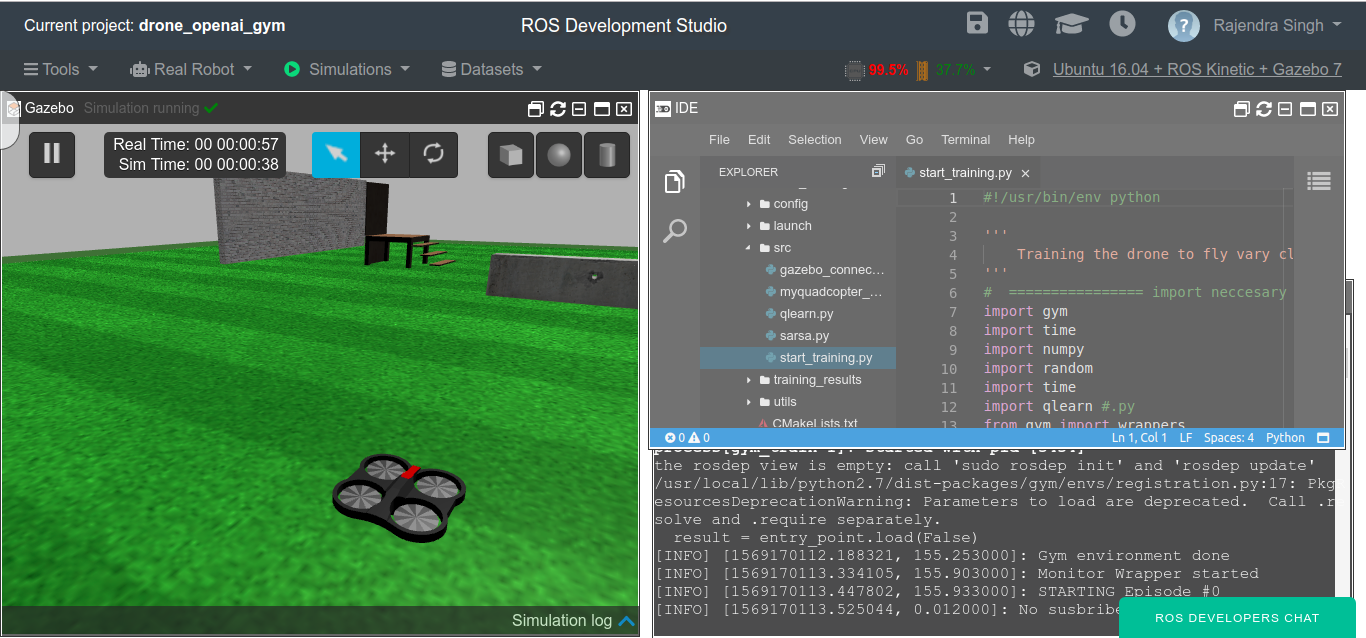
\includegraphics[width=\textwidth]{images/rds.png}
    \caption{Simulation of ARdrone on ROS Development studio}
\end{figure}





\subsection{Q-learning}
Below I present the pseudo code of Q-learning algorithm on ARdrone to training it to fly from point A to point B. Full detailed code of the same can be found \href{https://github.com/iamrajee/Slam_and_RL_BTP/tree/master/code/AI/drone}{here}.\cite{rosject}\\

\textbf{Pseudo Code}
\begin{minted}{python}
'''
    Training the drone to fly from point A to point B.
'''
#  ================ import necessary gym and ros libraries ============= #
if __name__ == '__main__':
    # ======= Create the Gym environment ===#
    # ============== Set the logging system ==================#
    # load param form yaml file
    # Initialises(class) the algorithm that we are going to use for learning
    # run for n episodes
        # ==== For n steps ====#
            action = qlearn.chooseAction(state) # Pick an action based on the current state
            observation, reward, done, info = env.step(action)# Execute the action in the environment and get feedback
            cumulated_reward += reward
            if highest_reward < cumulated_reward:#update the highest_reward
                highest_reward = cumulated_reward
            nextState = ''.join(map(str, observation)) #next state
            qlearn.learn(state, action, reward, nextState)# Make the algorithm learn based on the results
            if not(done):
                state = nextState
            else:
                break #done
    #publish ros log
    env.close() #close env

\end{minted}
% \newcommand{}[]{}
\textbf{Note:}\\
1.) In above code we import the myquadcopter-env.py, this is a openai gym environment made using ARdrone gazebo simulation and It is not written by me.



\subsection{Sarsa}
Implementing sarsa is also similar to q learning but here we will have different update function. Full detailed code of the same can be found \href{https://github.com/iamrajee/Slam_and_RL_BTP/tree/master/code/AI/drone}{here}.\\

\textbf{Pseudo Code}
\begin{minted}{python}


'''
    Here update rule also similar to that in q learning but a'(action to be taken from nextstate s' in each step in any episode) is chosen based epsilon greedy algorithm which is as  below s
'''
def chooseAction(self, state):
        if random.random() < self.epsilon:
            action = random.choice(self.actions)
        else:
            q = [self.getQ(state, a) for a in self.actions]
            maxQ = max(q)
            count = q.count(maxQ)
            if count > 1:
                best = [i for i in range(len(self.actions)) if q[i] == maxQ]
                i = random.choice(best)
            else:
                i = q.index(maxQ)

            action = self.actions[i]
        return action

\end{minted}

\subsection{Conclusion}
In this chapter, we proposed another algorithm to control the drone, which is based on the Q learning and Sarsa. As this task not just required the good understanding of Q learning but also required very good understanding of ROS and gazebo, ARdrone simulation and ros message and topics.
Hence, It was not possible for me to write whole code myself and therefore I used libraries for some part, e.g. myquadcopter-env.py as mentioned above. In future, I'll learn and try to write the env also myself.

